\documentclass{article}
\usepackage[utf8]{inputenc}
\usepackage[T1]{fontenc}
\usepackage[margin=0.7in]{geometry}
\usepackage{graphicx}
\usepackage{amsmath}
\usepackage{amssymb}
\usepackage{xcolor}
\usepackage{color}
\usepackage{listings}
\usepackage{minted}
\newcommand{\Stack}{\texttt{ArrayList<T> stack} }

\title{3S03 - Software Testing \\
Assignment 2}
\author{Mark Hutchison \\
hutchm6@mcmaster.ca \and
Jatin Chowdhary \\
chowdhaj@mcmaster.ca}
\date{\today}

\begin{document}

\maketitle

\tableofcontents

\section*{Question 1 - Prime Numbers}

\subsection*{Part A - Implementing Sieve Of Eratosthenes Algorithm}

The code below refactors the \texttt{PrimeNumber} class to calculate prime numbers using the \textit{Sieve of Eratosthenes} approach. However, the fault from before (i.e. False negatives) remains while introducing new faults (i.e. False positives).

\begin{lstlisting}[language=Java]
import java.util.ArrayList;
import java.util.Iterator;
import java.util.List;

/**
 * Reimplements the algorithm for calculating primes using the Sieve
 * of Eratosthenes, but leaves the fault from before in place. This
 * causes new issues like false positives, where a number that is not
 * a prime is added to the list of primes.
 *
 * The only change made to this lies in the for-loop. The condition
 * in the for loop, ``divisor <= number`` is changed to
 * ``(divisor * divisor) <= number`` to satisfy the Sieve of
 * Eratosthenes algorithm.
 *
 * @author  hutchm6
 * @author  chowdhaj
 * @course  SFWRENG 3S03
 * @version 1.1
 * @date    March 11th, 2022
 */
public class PrimeNumbersEratosthenes implements Iterable<Integer> {

    private List<Integer> primes = new ArrayList<Integer>();

    public void computePrimes(int n) {
        int count = 1; // count of primes
        int number = 2; // number tested for primeness
        boolean isPrime; // is this number a prime

        while (count <= n) {
            isPrime = true;
            // NOTE: This is where the change is; it is the only change
            for (int divisor = 2; (divisor * divisor) <= number / 2; divisor++) {
                if (number % divisor == 0) {
                    isPrime = false;
                    break; // for loop
                }
            }
            if (isPrime && (number % 10 != 9)) { // FAULT
                primes.add(number);
                count++;
            }
            number++;
        }
    }

    /**
     * Overrides the ``iterator()`` method
     */
    @Override
    public Iterator<Integer> iterator() {
        return primes.iterator();
    }

    /**
     * Overrides the ``toString()`` method to print all primes in the
     * List<Integer>
     */
    @Override
    public String toString() {
        return primes.toString();
    }
}

/*
---------------
DEPRECATED CODE
---------------
// NOTE: At the last minute I realized I did not need to over-
//       complicate the solution for "Sieve of Eratosthenes".
//       Shout-out to the TAs for their help!
//
//  boolean isPrime[] = new boolean[n]; // is this number a prime
//      Arrays.fill(isPrime, true);
//      for (int divisor = 2; divisor * divisor <= n; divisor++) {
//          if (isPrime[divisor]) {
//              for (int j = divisor; j * divisor < n; j++) {
//                  isPrime[j * divisor] = false;
//              }
//          }
//          if (isPrime[divisor] && (divisor % 10 != 9)) { // FAULT
//              primes.add(divisor);
//              count++;
//          }
//      }
//  }
*/
\end{lstlisting}

\subsection*{Part B - Identifying False Positives}

\smallskip

\begin{itemize}
    \item In the original algorithm, we encountered false negatives due to the fault that was purposely added via the following line: $(number \ \% \ 10 \ != 9)$. After modifying the algorithm to solve prime numbers via \textit{Sieve of Erathosthenes}, we now have false positives. False positives arise when a non-prime number enters the list of prime numbers - it makes its way to the final list of prime numbers. Evidently, this is incorrect and not the intended behavior of our program/algorithm.
    \item The first false positive generated by our \textit{Sieve of Erathosthenes} algorithm occurs when \texttt{number=4}. The number 4 is not a prime number because it is divisible by 2 in addition to being divisible by 1 and itself. After 2 numbers (i.e. 2 and 3), or two test cases, is when our \textit{Sieve of Erathosthenes} algorithm generates a false positive, 4.
    \item Let's analyze the the conditions for the first 3 numbers (or test cases) to understand exactly why this false positive occurs. \textit{Note: The explanation is provided in the code itself}.

\end{itemize}

\begin{enumerate}

    \item First Test Case (When \texttt{number=2}):

    \begin{lstlisting}[language=Java]
    int n = 100;
    int count = 1;
    int number = 2;
    boolean isPrime;

    while (count <= n) { // Checks if (1 <= 100)
        isPrime = true;
        // Checks if ((2 * 2) <= (2 / 2)) // Evaluates to false
        for (int divisor = 2; (divisor * divisor) <= number / 2; divisor++) {
            if (number % divisor == 0) {
                isPrime = false;
                break; // for loop
            }
        }
        // Since for-loop does not execute, 'isPrime' is true
        if (isPrime && (number % 10 != 9)) { // FAULT
            primes.add(number); // Add 2 to list of primes
            count++; // Counter is now 2
        }
        number++; // Number is now 3
    }
    \end{lstlisting}

    \item Second Test Case (When \texttt{number=3}):

    \begin{lstlisting}[language=Java]
    int n = 100;
    int count = 1;    // count is now 2
    int number = 2;   // number is now 3
    boolean isPrime;

    while (count <= n) { // Checks if (2 <= 100)
        isPrime = true;
        // Checks if ((2 * 2) <= (3 / 2)) // Evaluates to false
        for (int divisor = 2; (divisor * divisor) <= number / 2; divisor++) {
            if (number % divisor == 0) {
                isPrime = false;
                break; // for loop
            }
        }
        // Since for-loop does not execute, 'isPrime' is true
        if (isPrime && (number % 10 != 9)) { // FAULT
            primes.add(number); // Add 3 to list of primes
            count++; // Counter is now 3
        }
        number++; // Number is now 4
    }
    \end{lstlisting}

    \item Third Test Case (When \texttt{number=4})
    \textit{This is where the false positive occurs}:

    \begin{lstlisting}[language=Java]
    int n = 100;
    int count = 1;    // count is now 3
    int number = 2;   // number is now 4
    boolean isPrime;

    while (count <= n) { // Checks if (3 <= 100)
        isPrime = true;
            // Checks if ((2 * 2) <= (4 / 2)) // Evaluates to false
            //                 (4 <= 2)
            //                 (false)
            for (int divisor = 2; (divisor * divisor) <= number / 2;
                 divisor++) {

            if (number % divisor == 0) {
                isPrime = false;
                break; // for loop
            }
        }

        // Since for-loop does not execute, 'isPrime' is true, and
        // this is where the false positive occurs, because the
        // condition in the for-loop evaluates to false
        if (isPrime && (number % 10 != 9)) { // FAULT
            primes.add(number); // Add 4 to list of primes // WRONG
            count++; // Counter is now 4
        }

        number++; // Number is now 5
    }
    \end{lstlisting}

    \end{enumerate}

\begin{itemize}

    \item The second false positive occurs when \texttt{number=6}. We know that 6 is not a prime number, yet it is wrongly added to the list of primes. The number 6 is not a prime number because its factors are: \textit{[1, 2, 3, 6]}. Clearly, 6 is not a prime number. Hence, the second false positive occurs at the 5th test case or iteration. The reason for this false positive is similar to the first false positive that is generated at the 3rd test case or iteration - the condition (wrongly) evaluates to false.

    \item Note: We are not including the false negatives that exist due to the inherent nature of the program due to $(number \ \% \ 10 \ != 9)$. This is a completely separate issue. The issue caused by this are false negatives; failure to include a prime number \textit{(i.e. 19, 29, etc.)}

\end{itemize}

\subsection*{Part C - Mutation Testing (aka \texttt{RIPF} Model)}

\begin{enumerate}

    \item \textbf{Reachable:} The reimplemented algorithm, based on \textit{Sieve of Eratosthenes} contains two faults; a false positive and a false negative:

       \begin{enumerate}

            \item \texttt{for (int divisor = 2; (divisor * divisor) <= number / 2; divisor++)\{\}}

            \begin{itemize}
                \item This fault generates a false positive. Non-prime numbers (i.e. 4) are added to the list of prime numbers; illustrated in part \textit{1B}.
            \end{itemize}

            \item \texttt{if (isPrime \&\& ($number \ \% \ 10 \ != 9$)) \{\}}

                \begin{itemize}
                    \item This fault generates a false negative. Prime numbers (i.e. 19) are not added to the list of prime numbers.
                \end{itemize}

        \end{enumerate}

    Running the reimplemented program can lead to one of, or both, faults; stated above - assuming the program runs for a minimum number of iterations (identified to be 4 in part \textit{1B}.)

    \item \textbf{Infection:} After one, or both, of the faulty locations are executed, the state of the program is incorrect/infected. This is because the infected state propagates through the execution and causes the output - the list of prime numbers - to be incorrect. Once the program reaches a minimum number of 3 iterations (or test cases), we can automatically assume that the program has reached an incorrect/infected state. Furthermore, the list of prime numbers can be considered as \textit{stored data}, which gets infected/contaminated once the program reaches the faulty location(s).

    \item \textbf{Propagation:} The faulty locations in the algorithm result in an infected state which propagates through the execution and causes some output of the final state of the program to be incorrect/infected. We observe this by analyzing the output of the program: \textit{[2, 3, 4, 5, 6, 7, 11, 13, 15, 17, 23, ... ]}. As you can see, the following numbers do not belong, because they are not prime numers: \textit{[4, 6, 15, ... ]} - these are false positives. In addition, the following numbers are missing: \textit{[19, 29, ... ]} - these are false negatives. Therefore, the final state of the program is incorrect/infected, due to the faulty locations mentioned above.

    \item \textbf{Revealing:} Users, developers, and testers can effortlessly observe that the final state of the program is infected - more specifically, incorrect. Upon manually analyzing the output, it is highly apparent that several numbers are incorrectly added (i.e. false positives), and several numbers have not been added (i.e. false negatives). Even though revealability is high for manual testing, it is quite low for automated testing. In other words, there is no test case/suite that can determine if the calculations performed by the program/algorithm are correct or not. The program/algorithm is allowed to continue in an infected/incorrect state, without being noticed by the stakeholders of the program.

        \begin{itemize}
            \item Note: For this particular algorithm, the results produced by the program can be verified through automated testing. The process is quite tedious but involves something like feeding the output from the \textit{Sieve of Eratosthenes} algorithm into another algorithm that has been mathematically proven to (efficiently) compute prime numbers \textit{(i.e. AKS Primality Test)}. While this approach works for this particular example, it fails for others. For instance, there are no known solutions to solving discrete logarithms on elliptic curves. In this situation, testing is (inherently) manual, with no automation.
        \end{itemize}

\end{enumerate}

This example demonstrates that testing is complicated and comes with a plethora of technical issues. In terms of reachability, faulty locations in code may or may not be executed. For instance, if the input is constant, then we can predict if the final state of the program will be infected/incorrect or not. However, most input is unpredictable - we do not know what the user may or may not submit. In addition, it is very difficult for automated testing to determine if the infected state has propagated through the execution and caused some output of the final state of the program to be incorrect. This lowers revealability, making testing more cumbersome, complicated, and tedious. In conclusion, testing is very complicated!

\section*{Question 2 - Partition Testing}

\subsection*{Part A - List all input variables}

\begin{enumerate}
    \item The GenericStack class must contain an \Stack inside it to store the elements we push to it, and an indicator of what element in the \texttt{stack} is currently being pointed to as the top element. Thus, the constructor takes in no parameters, and instead only initializes these state variables. However, the constructor does take in one item of interest: \texttt{<T>}. A type must be instantiated at that point, which is relevant to the \texttt{Object} type later on.
    \item The \texttt{push} method takes in one parameter, \texttt{Object x}, and pushes it onto the \texttt{stack}. This modifies the state of the \texttt{top} and \texttt{stack} variables, as well as accepts the input of \texttt{x}.
    \item The \texttt{pop} method takes in no parameters, and pops the top element off the \texttt{stack}. This modifies the state of the \texttt{top} and \texttt{stack} variables, as well as returns the popped element, meaning the return type is \texttt{<T>} (type \texttt{Object}).S
    \item The \texttt{isEmpty} method takes in no parameters, and returns a boolean value, indicating whether or not the \texttt{stack} is empty. This does not modify the state of the \texttt{top} and \texttt{stack} variables, nor return anything but a simple boolean.
\end{enumerate}

\subsection*{Part B}

\begin{enumerate}
    \item
    \begin{itemize}
        \item \Stack can either either be occupied or empty. However, I argue having ``occupied'' being split into two blocks is more helpful than a binary split. I propose we split the ``occupied'' block into two blocks, one for a stack of 1 element, and one for a stack of 2 or more elements. The reason is that a stack of one element becomes empty when it is popped, and a stack of 2 or more elements does not, which is a distinct and testable condition.
        \item Everything above relies on a soul construct though: \Stack exists in the first place. What if it is constructed as an NULL stack? Not the same as an empty stack, for it doesn't even have a stack-like value.
        \item The constructor itself takes in no arguments and thus can't actually be partitioned. However, via state mutation techniques, nothing stops us from partitioning the \Stack as mentioned above. It is just unlikely to occur through normal partition testing alone.
    \end{itemize}
    \item
    \begin{itemize}
        \item Push takes in a generic Object, but who is to say that the Object is of type \texttt{T}? I propose we split our partitions first into two blocks: object is of type \texttt{T}, and object is not of type \texttt{T}. For objects not of type \texttt{T}, we can't push them onto the stack, so we would expect errors to be thrown during testing. For objects of type \texttt{T}, we can push them onto the stack, and we would expect no errors to be thrown during testing. Additionally, the size of the stack should be growing consistently during the push operation, and we could test for that. Sadly, we can't further partition either of the blocks since we know too little about the type of the object.
        \item The state is being naturally mutated during the push operation, and we can test for that. We can test pushing onto an empty stack to see that it becomes non-empty, as well as pushing onto a non-empty stack to verify that the size of the stack is growing. Apart from that, further partitioning would be pointless.
        \item If the \Stack is null, attempting to push would result in an error, so test this block too!
    \end{itemize}
    \item
    \begin{itemize}
        \item Pop deals with the \Stack directly, meaning that expecting errors isn't as reasonable. However, because the state of the stack can be empty, we do have one potential error. We should run pop on an empty stack to verify the behavior is as expected.
        \item From their, as mentioned in my first point, I believe the partition of the occupied stack should be further split into two blocks. The stack of one element would become an empty stack, which can be tested for. The stack of 2 or more elements would not, and thus we can test for that. Both of these tests would facilitate using \texttt{isEmpty} to test for emptiness, which is different for these two stacks.
        \item If the \Stack is null, attempting to pop would result in an error, so test this block too!
    \end{itemize}
    \item
    \begin{itemize}
        \item The function \texttt{isEmpty} relies entirely on the state of the stack in two universes: the occupied and empty universes. There is not much difference in the two universes, so I would leave the stack state partitions at simply Empty Stack and Non-Empty Stack for testing purposes.
        \item If the \Stack is null, what would \texttt{isEmpty} return? This should be explicitly tested.
    \end{itemize}
\end{enumerate}

\subsection*{Part C}

Now that we have our descriptions from above, here are my blocks better defined and stated. I am assuming mutation testing is possible for the constructor, but if it isn't, than there is nothing in your control as a developer to test and thus no blocks.
\begin{enumerate}
    \item Constructor: The only way to modify the partition of the \Stack during construction is to play with Mutation Testing. Via this method, we can establish the partition of the \Stack to be NULL, Empty, Non-Empty. There is no need to further partition the Non-Empty block due to lack of change in behavior.
    \item Push:
    \begin{itemize}
        \item Object: Partition your Object domain into three blocks: NULL of type \texttt{T}, Object of type \texttt{T}, and Object of type \texttt{!T}. For objects of type \texttt{T}, we can push them onto the stack, and we would expect no errors to be thrown during testing. For objects of type \texttt{!T}, we can't push them onto the stack, so we would expect errors to be thrown during testing. A NULL of type \texttt{T} is interesting because technically it is allowed on the stack due to meeting type checks. Although the behavior is the same, the edge case is interesting enough to earn its own block. Additionally, the size of the stack should be growing consistently during the push operation, and we could test for that as well.
        \item Stack: You can have your stack constructed as NULL and expect errors to be thrown during testing. Meanwhile, Empty and Non-Empty both operate the exact same way, so you can simply combine those into a Not-NULL block if you wanted.
    \end{itemize}
    \item Pop: The 4 main \Stack partitions should be used here, as each behaves differently to one-another:
    \begin{itemize}
        \item NULL cannot be popped and should error
        \item Empty cannot be popped, but you may not error and you may just return a NULL object or something
        \item Non-Empty 1 Element can be popped, and should become Empty after popping
        \item Non-Empty 2+ Elements can be popped, and should remain Non-Empty after popping
    \end{itemize}
    Pop always returns an Object, but the object must be of type T since it exists on the stack.
    \item isEmpty: Again, this can be done through mutation testing or utilizing earlier methods. Our aim is to build the standard stack partitions of NULL, Empty, Non-Empty. The Non-Empty can be further partitioned like in pop, but there is little reason due to the lack of change in behavior.
\end{enumerate}

\subsection*{Part D}

Since a lot of the partitions are repeated, I am going to simply going to use the Block names from above for each of the block values:

\begin{itemize}
    \item \Stack
    \begin{itemize}
        \item NULL: \texttt{ArrayList<T> stack = NULL;}
        \item Not-NULL: $\text{Empty}\ \cup\ \text{Non-Empty}$
        \item Empty: \texttt{ArrayList<T> stack = new ArrayList<T>();}
        \item Non-Empty:  $\text{Non-Empty 1 Element}\ \cup\ \text{Non-Empty 2+ Element}$
        \item Non-Empty 1 Element: \texttt{ArrayList<T> stack = new ArrayList<T>(); stack.add(new T());}
        \item Non-Empty 2+ Element: \texttt{ArrayList<T> stack = new ArrayList<T>(); stack.add(new T()); stack.add(new T()); ...}
    \end{itemize}
    \item Push - Object
    \begin{itemize}
        \item Object of type \texttt{T}: \texttt{Object x = new T();}
        \item NULL of type \texttt{T}: \texttt{Object x = NULL;} if NULL is a valid term of type T
        \item Object not of type \texttt{T}: \texttt{Object x = new Y();} where Y is not of type T
    \end{itemize}
    \item Pop - Object: Returned Object must be of type T
    \begin{itemize}
        \item Object of type \texttt{T}: \texttt{Object x = new T();}
        \item NULL of type \texttt{T}: \texttt{Object x = NULL;} if NULL is a valid term of type T and is expected on \texttt{pop} Empty.
    \end{itemize}
\end{itemize}

\section*{Question 3 - Control Flow Graphs}

\subsection*{Part A - The Control Flow Graph}

% Include image from img folder
\begin{figure}[htbp]
    \centering
    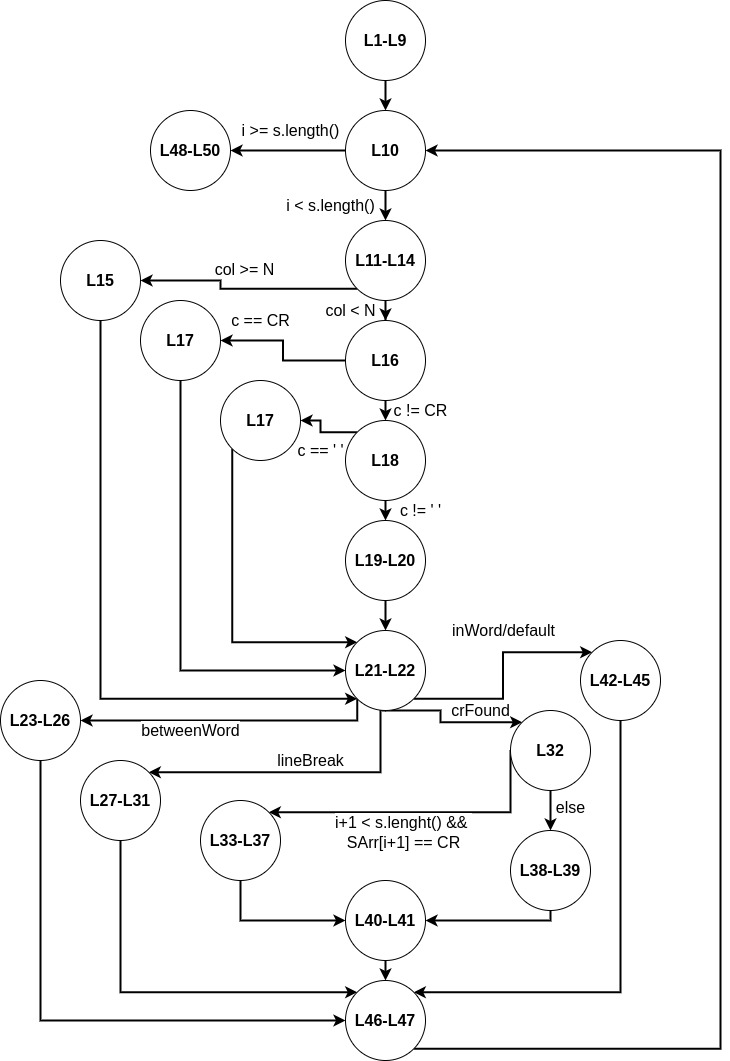
\includegraphics[width=0.8\textwidth]{./img/3S03-A2-Q3-P1.jpg}
    \caption{Control Flow Graph}
    \label{fig:CFG}
\end{figure}

\subsection*{Part B - Skipping the Loop}

Looking at the CFG attached, we can see that we have an edge from the while loop to the end of the method when $i \ge s.length()$. Since $i = 0$, the only option we have is to set input $s = ``''$ in order to fail the while condition. Now, I also thought about using an input of $s = NULL$ (or whatever equivalent) instead of empty string, but that doesn't work because $NULL$ wouldn't have a length and would trigger an error. An error may cause the program to halt, but not complete, which isn't what the question is asking for.

\subsection*{Part C - Requirements for Coverage}

\subsubsection*{Part C.1 - Requirements for Node Coverage}

Our nodes are denoted by the lines of code that run from each node. Thus, full node coverage means full statement coverage (under this specific graph), which means our test cases need to get into every line of code. Requirements to do that:

\begin{itemize}
    \item Input must be a string greater than length 0. A string of length 0 hits nodes already covered by this positive test case.
    \item The if statement has multiple nodes that are exclusive, but I think we can construct single string that would cover all of them over the several loops that occur.
    \begin{itemize}
        \item Have a string greater than length N
        \item String contains the manual line break character
        \item String has at minimum one space between words.
        \item String contains letters before index N that aren't spaces.
    \end{itemize}
    \item Because we hit each if statement, we hit each switch statement case too. However, we have a new if statement to deal with: Two newlines back to back.
    \begin{itemize}
        \item Make it so the input string has both a single newline character and a double newline character within it while obeying above rules.
    \end{itemize}
    \item The while loop ends, guaranteeing access to final node.
\end{itemize}

Following the above requirements, we can construct a single test case that will cover all nodes. Something like:

\texttt{FmtRewrap.fmtRewrap(``This is \textbackslash n a\textbackslash n\textbackslash n test.'', 9)}

\subsubsection*{Part C.2 - Requirements for Edge Coverage}

At no point is there ever two different edges connecting the same nodes on the graph. If we end up going to a node, we have to take both the input and output edge associated with that node. Thus, the same test case given for node coverage would also cover the edge coverage. Because we have to hit nodes \texttt{L23-L26}, \texttt{L27-L31}, \texttt{L32}, \texttt{L42-L45}, we end up covering all 4 of the connecting edges, and all of the output edges for the same reason.

\texttt{FmtRewrap.fmtRewrap(``This is \textbackslash n a\textbackslash n\textbackslash n test.'', 9)}

\subsubsection*{Part C.3 - Requirements for Prime Coverage}

There are going to be an utter butt-ton of prime paths with how many nodes this graph has. But, we can address some specific cases that reduce the number.

\begin{itemize}
    \item No prime path starting at line 1 will be able to go through the loop multiple times. We will hit the loop entrance numerous times and thus would break. Thus, our test cases can't loop multiple times.
    \item If we hit a switch statement, because we hit the entrance numerous times, we once again can't have multiple loops at this part.
    \item Prime paths can be constructed mid-graph though, so we can have a prime path that starts during a case statement and then loops back to the same case, or even a different case statement.
\end{itemize}

Basically, because prime paths can start at any node, my "reduce" points are basically useless. These paths are rather long, covering each unique path linearly down the graph. I would argue that the minimum number of paths is $O(|V| \cdot |E|)$, which is $O(19 \cdot 26)$ which is a minimum of 496 paths! Jeez!


\end{document}
